\documentclass[withoutpreface]{cumcmthesis}

\begin{document}

\begin{abstractpage}{线性回归分析简介}

  本文主要研究线性回归分析的基本知识。

  首先,我们简述了什么是回归分析,借此引入了线性回归分析。其次,我们从多方面简单地介绍线性回归分析的原理和应用。最后,我们以高数成绩的线性回归为例,展示了线性回归的基本应用步骤。

  值得注意的是,本文只提到了线性回归分析的简单应用。其它诸如异方差、多重共线性、显著性检验等具有一定理解难度的知识并未提及。
  


  \keywords{回归 \quad 线性 \quad 共生性 \quad 因变量 \quad 自变量}
\end{abstractpage}

\tocpage

\section{回归分析简介}
\textbf{回归分析}是数据分析中最基础也是最重要的分析工具,绝大多数的数据分析问题,都可以使用回归的思想来解决。回归分析的基本任务是,通过研究自变量 X 和因变量 Y 的相关关系,尝试去解释 Y 的形成机制,进而达到通过 X 去预测 Y 的目的。

回归分析的基本任务中,包含着三个重要因素:\textbf{自变量} X 、\textbf{因变量} Y 、\textbf{相关关系}。

数据间的因果关系是很难进行探究和验证的,我们往往只能退而求其次,根据经验和问题的驱动,提前假定某些变量为因变量,某些变量为自变量,研究它们的相关程度,以近似因果程度。

自变量是我们要研究的某一问题的因素变量,它在某一程度上影响着因变量的变化。因变量是那些我们认为受自变量影响的变量。按照另一种理解, X 为解释变量, Y 为被解释变量。

按照因变量 Y 的数值类型,可以对回归任务进行分类。本文主要研究线性回归。

\begin{table}[H]
  \centering
  \caption{回归任务分类}
  \begin{tabular}{|c|c|c|c|}
    \hline
    \textcolor[rgb]{ .267,  .329,  .416}{\textbf{类型}} & \textcolor[rgb]{ .267,  .329,  .416}{\textbf{模型}} & \textcolor[rgb]{ .267,  .329,  .416}{\textbf{自变量数值类型}} & \textcolor[rgb]{ .267,  .329,  .416}{\textbf{实例}} \bigstrut \\
    \hline
    \rowcolor[rgb]{ .851,  .882,  .949} 线性回归          & 最小二乘法                                             & 连续型变量                                                  & GDP ,产量,收入 \bigstrut                                        \\
    \hline
    \rowcolor[rgb]{ .851,  .882,  .949} 0-1回归         & Logistic 回归                                       & 二值0-1变量                                                & 是否 \bigstrut                                                \\
    \hline
    \rowcolor[rgb]{ .851,  .882,  .949} 定序回归          & probit 定序回归                                       & 定序变量                                                   & 优良差等级评定 \bigstrut                                           \\
    \hline
    \rowcolor[rgb]{ .851,  .882,  .949} 计数回归          & 泊松回归                                              & 计数变量                                                   & 每分钟车流量 \bigstrut                                            \\
    \hline
    \rowcolor[rgb]{ .851,  .882,  .949} 生存回归          & Cox 等比例风险回归                                       & 生存变量(截断型数据)                                            & 产品寿命 \bigstrut                                              \\
    \hline
  \end{tabular}
\end{table}

\section{线性回归}

\subsection{线性回归的形式}
线性回归的一般形式为
\begin{equation}\label{Eq:1}
  y = \theta_0 + \theta_1x_1+\theta_2x_2+\cdots+\theta_nx_n+ \mu
\end{equation}

其中,$\theta_i(i=1,2,\cdots,n)$称为自变量$x_i$的\textbf{回归系数}。$\mu$为误差项。$\theta_0$称为截距,它代表自变量取值全为0时因变量的估计值。

线性回归的任务是找到参数$\theta_i$使得误差项$\mu$尽量小。

\subsection{广义线性}

将\cref{Eq:1}中的$x_i$全部或部分改为不含参数的$g_i(x_i)$,线性回归也能进行。

\subsection{最小二乘法}

线性回归常常使用最小二乘法求解参数,即最小化$\frac{1}{2}\mu^2$。

若已知数据$X = \begin{bmatrix}
    1 & x_1^{(1)} & x_2^{(1)} & \cdots & x_n^{(1)} \\
    1 & x_1^{(2)} & x_2^{(2)} & \cdots & x_n^{(2)} \\
    1 & \vdots    &           &        & \vdots    \\
    1 & x_1^{(m)} & x_2^{(m)} & \cdots & x_n^{(m)} \\
  \end{bmatrix}$,
$y=\begin{bmatrix}
    y^{(1)} \\
    y^{(2)} \\
    \vdots  \\
    y^{(m)}
  \end{bmatrix}$,

并设
$\theta=\begin{bmatrix}
    \theta_0 \\
    \theta_1 \\
    \vdots   \\
    \theta_n\end{bmatrix}$,
$\mu=\begin{bmatrix}
    \mu^{(1)} \\
    \mu^{(2)} \\
    \vdots    \\
    \mu^{(m)}\end{bmatrix}$,则
\begin{equation}\label{Eq:2}
  cost(\theta)=\frac{1}{2}\mu^T\mu=\frac{1}{2}         (X\theta-y)^T(X\theta-y)=\frac{1}{2}[\theta^TX^TX\theta-2\theta^TX^Ty+y^Ty]
\end{equation}

\cref{Eq:2}两边对$\theta$求偏导,得到
\begin{equation}
  \frac{\partial{cost(\theta)}}{\partial{\theta}}=X^TX\theta - X^Ty
\end{equation}

假设$X^TX$可逆,解得
\begin{equation}
  \theta = (X^TX)^{-1}X^Ty
\end{equation}


\vspace{-0.8cm}
\subsection{内生性的影响}
\vspace{-0.2cm}
\cref{Eq:1}中的$\mu$代表无法观测的扰动误差项。如果$\mu$与所有的自变量$x_i$均不相关,则称该回归模型具有\textbf{外生性}。否则,则称该回归模型具有\textbf{内生性}。具有内生性的回归模型,由于扰动误差项$\mu$包含与已解释自变量相关的其他变量的信息,不满足无偏和一致性,将导致回归系数估计的不准确。

如果考虑的自变量数目过少,模型就容易产生内生性。

我们以$y=1+2x_1+3x_2+\mu$为例,进行蒙特卡洛模拟实验。假设其中的$\mu$服从$N(0,1)$,而$x_2$与$x_1$相关,以$y'=b+kx_1+\mu'$进行线性回归,同时记录$\mu' = \mu + 3x_2$与$x_1$之间的相关系数$r_{x_1,\mu'}$和$k$值大小,得到\cref{Fig:1}。

\begin{figure}[H]
  \centering
  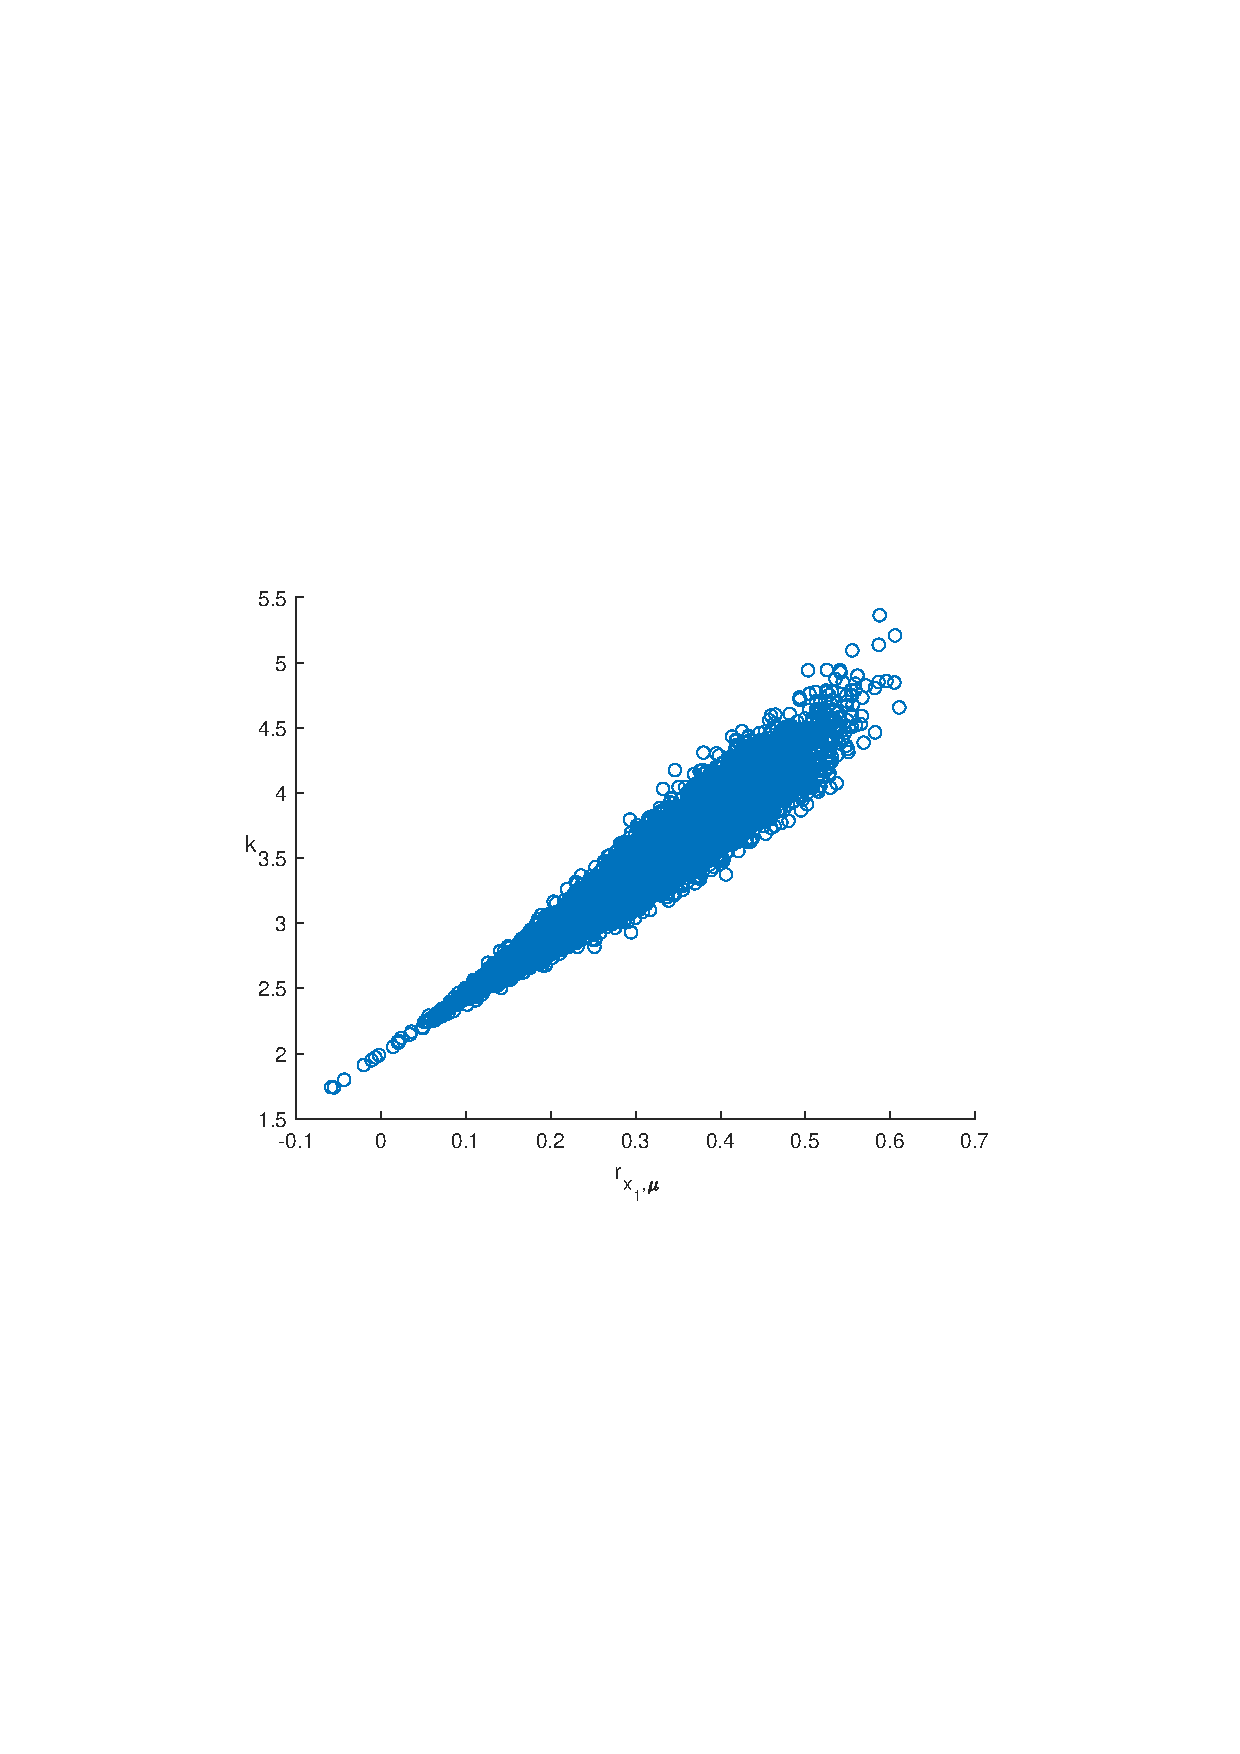
\includegraphics[width=0.42\textwidth]{内生性}
  \vspace{-0.3cm}
  \caption{内生性对回归系数的影响}\label{Fig:1}
\end{figure}

由\cref{Fig:1}可见,当扰动误差项$\mu'$中包含我们遗漏的与$x_1$相关的变量$x_2$时,常常导致$\mu'$与$x_1$相关性较大,我们估计的$x_1$的回归系数$k$与真实值有较大偏差。

无内生性 (no endogeneity) 要求所有解释变量均与扰动误差项不相关。这个假定通常太强,因为解释变量一般很多,很难保证它们全都与扰动误差项不相关。不过,我们对这个条件进行适当的减弱。把解释变量区分为\textbf{核心解释变量}与\textbf{控制变量}两类。

\textbf{核心解释变量}:我们最感兴趣的变量,因此我们特别希望得到对其回归系数的一致估计(当样本容量无限增大时,收敛于待估计参数的真值 )。

\textbf{控制变量}:我们可能对于这些变量本身并无太大兴趣;而之所以把它们也放入回归方程,主要是为了 “控制住” 那些对被解释变量有影响的遗漏因素,为了防止遗漏与核心解释变量相关的其他因素。

在实际应用中,我们只要保证核心解释变量与$\mu$不相关即可,即在解释变量中尽可能多地列出与核心变量相关的控制变量。

\subsection{设置交互项}

如果两个自变量$x_i,x_j$之间存在着相互影响各自对因变量的影响的关系,我们可以设置交互项$x_ix_j$。

原本有$\frac{\partial y}{\partial x_i}=\theta_i$,加入交互项$x_ix_j$后$\frac{\partial y}{\partial x_i} = \theta_i+\theta_{ij}x_j$,即$x_j$的大小将影响$x_i$对于$y$的影响。

\subsection{标准化线性回归}

如果在进行线性回归之前,对连续型自变量和因变量进行标准化,即:

\begin{equation}
  x' = \frac{x-Mean(x)}{Std(x)}
\end{equation}

我们便可以通过比较回归系数的大小来判断各因变量对自变量的影响程度。

\section{简单示例}

给出20位同学的高数成绩及相关数据如。请就高考成绩、学年平均绩点、性别(0代表女生,1代表男生)三个因素对高数成绩进行线性回归分析。(该数据伪造而成,并不具有现实意义)。

\begin{table}[H]
  \centering
  \caption{20名同学的高数成绩及相关数据}
    \begin{tabular}{|c|c|c|c|}
    \hline
    \rowcolor[rgb]{ 1,  .753,  0} \textcolor[rgb]{ 1,  1,  1}{高考数学成绩} & \textcolor[rgb]{ 1,  1,  1}{学年平均绩点} & \textcolor[rgb]{ 1,  1,  1}{性别} & \textcolor[rgb]{ 1,  1,  1}{高数成绩} \bigstrut\\
    \hline
    \rowcolor[rgb]{ .859,  .859,  .859} 120   & 3.7   & 1     & 90 \bigstrut\\
    \hline
    \rowcolor[rgb]{ .929,  .929,  .929} 102   & 3.2   & 0     & 83 \bigstrut\\
    \hline
    \rowcolor[rgb]{ .859,  .859,  .859} 145   & 3.4   & 1     & 93 \bigstrut\\
    \hline
    \rowcolor[rgb]{ .929,  .929,  .929} 90    & 3.1   & 1     & 88 \bigstrut\\
    \hline
    \rowcolor[rgb]{ .859,  .859,  .859} 125   & 3.2   & 0     & 94 \bigstrut\\
    \hline
    \rowcolor[rgb]{ .929,  .929,  .929} 145   & 2.9   & 1     & 76 \bigstrut\\
    \hline
    \rowcolor[rgb]{ .859,  .859,  .859} 132   & 3.3   & 0     & 90 \bigstrut\\
    \hline
    \rowcolor[rgb]{ .929,  .929,  .929} 110   & 3.2   & 0     & 82 \bigstrut\\
    \hline
    \rowcolor[rgb]{ .859,  .859,  .859} 92    & 3.3   & 1     & 74 \bigstrut\\
    \hline
    \rowcolor[rgb]{ .929,  .929,  .929} 80    & 2.4   & 1     & 62 \bigstrut\\
    \hline
    \rowcolor[rgb]{ .859,  .859,  .859} 99    & 3.1   & 0     & 79 \bigstrut\\
    \hline
    \rowcolor[rgb]{ .929,  .929,  .929} 110   & 3.4   & 1     & 82 \bigstrut\\
    \hline
    \rowcolor[rgb]{ .859,  .859,  .859} 99    & 2.7   & 1     & 71 \bigstrut\\
    \hline
    \rowcolor[rgb]{ .929,  .929,  .929} 140   & 3.5   & 0     & 92 \bigstrut\\
    \hline
    \rowcolor[rgb]{ .859,  .859,  .859} 120   & 2.7   & 0     & 81 \bigstrut\\
    \hline
    \rowcolor[rgb]{ .929,  .929,  .929} 100   & 3.2   & 1     & 81 \bigstrut\\
    \hline
    \rowcolor[rgb]{ .859,  .859,  .859} 89    & 3.3   & 0     & 76 \bigstrut\\
    \hline
    \rowcolor[rgb]{ .929,  .929,  .929} 88    & 2.1   & 1     & 59 \bigstrut\\
    \hline
    \rowcolor[rgb]{ .859,  .859,  .859} 123   & 3.4   & 0     & 88 \bigstrut\\
    \hline
    \rowcolor[rgb]{ .929,  .929,  .929} 126   & 3.2   & 1     & 82 \bigstrut\\
    \hline
    \end{tabular}
  \label{Tab:2}
\end{table}

直接进行线性回归得到高数成绩(y)与高考数学成绩($x_1$)、学年平均绩点、性别($x_3)$之间的关系:
\begin{equation}
  y = 0.1711 x_1 +  15.3724 x_2  -3.1301 x_3 + 15.8701
\end{equation}

可以这样解释回归系数:学年平均绩点和性别相同时,高考数学成绩每相差10分,高数成绩平均相差1.711分;高考数学成绩和性别相同时,学年平均绩点每相差0.1,高数成绩平均相差1.53724分;高考数学成绩和学年平均绩点相同时,男同学的高数成绩比女同学平均要低3.1301分。

为了探知三个因素中,哪个因素对高数成绩的影响最大,可以进行标准化的线性回归,得到回归方程:
\begin{equation}
  y = 0.3561 x_1 +  0.6158 x_2  -0.1665 x_3
\end{equation}

可知,学年平均绩点对高数成绩的影响最大。

我们还可以通过可视化观察回归的误差,如\cref{Fig:2}所示。
\begin{figure}[H]
  \centering
  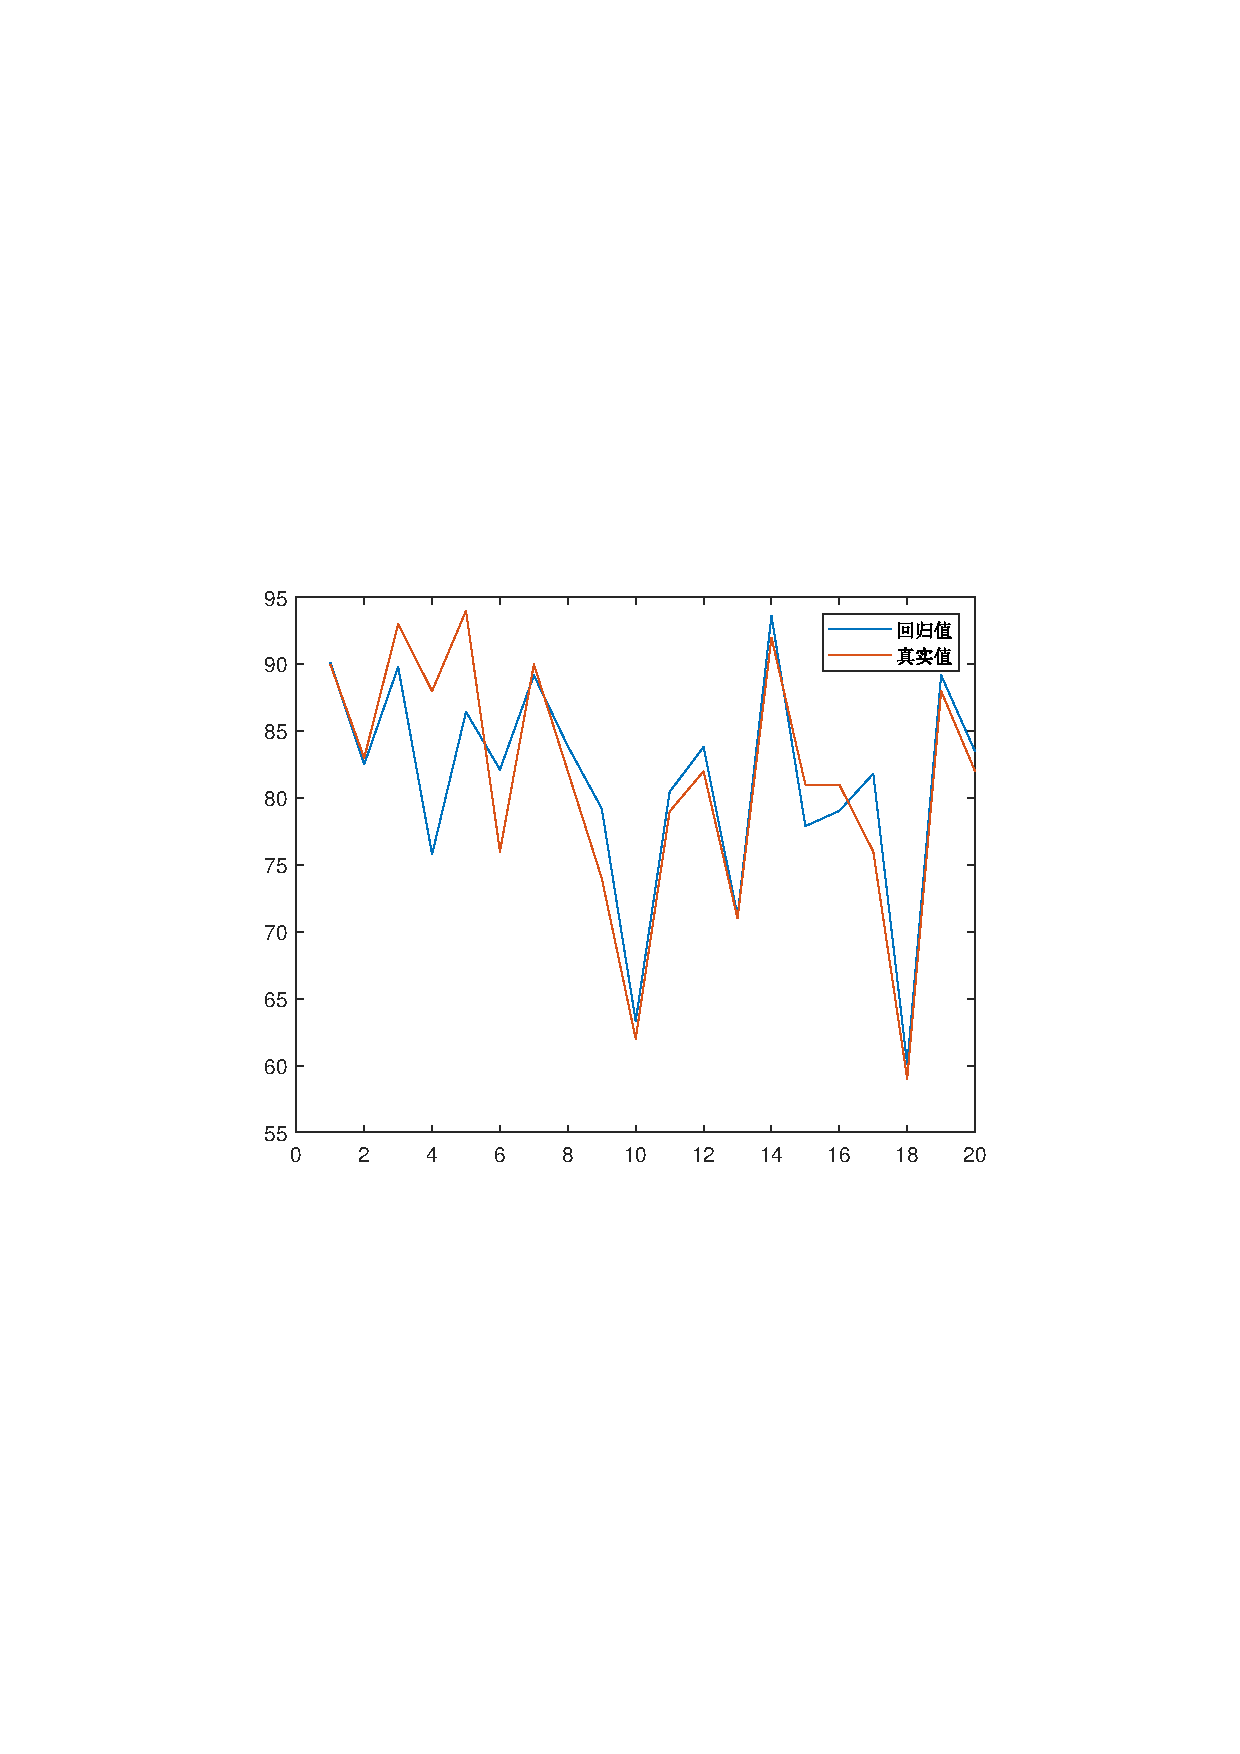
\includegraphics[width=0.8\textwidth]{线性回归分析}
  \caption{线性回归的效果}\label{Fig:2}
\end{figure}

\appendix
\section{Matlab代码}
  \begin{lstlisting}[language=matlab,caption={蒙特卡洛模拟}]
  clc,clear

  % 构造数据的函数
  f=@(x1,x2) 2*x1+5*x2+0.5;
  % 蒙特卡洛模拟次数
  times = 10000;
  n = 100;
  
  % 记录相关系数和回归系数
  r = ones(times,1);
  k = ones(times,1);
  for i=1:times
      % 随机数据x1
      x1 = -10+rand(n,1)*20;
      % 与x1相关的遗漏变量x2
      x2 = 0.3*x1+5*randn(size(x1,1),1);
      % 原扰动误差
      u0 = randn(n,1);
      y = f(x1,x2)+u0;
      % 遗漏变量x2进行回归
      theta = LinearRegression(x1,y);
      % 现扰动误差
      u1 = u0+5*x2;
      tmp = corrcoef(x1,u1);
      r(i) = tmp(1,2);
      k(i) = theta(2);
  end
  
  %% 绘图
  scatter(r,k);
  xlabel("r_{x_1,\mu}","Interpreter","tex");
  ylabel("k",Interpreter="tex",Rotation=0);
  \end{lstlisting}

  \begin{lstlisting}[language=matlab ,caption={自定义的线性回归函数} ]
  function [theta,values] = LinearRegression(X,y)
  % 线性回归
      X = [ones(size(X,1),1),X];
      theta = (transpose(X)*X)\transpose(X)*y;
      values = X*theta;
  end
  \end{lstlisting}

  \begin{lstlisting}[language=matlab ,caption={线性回归简单示例} ]
clc,clear

%% 读取数据
data = readmatrix("data\高数成绩.csv","NumHeaderLines",1);
X = data(:,1:3);
y = data(:,4);

%% 普通线性回归
[theta,values] = LinearRegression(X,y);
disp(theta);

%% 标准化线性回归
norm_X = normalize(X,1,"zscore");
norm_y = normalize(y,1,"zscore");
norm_theta = LinearRegression(norm_X,norm_y);
disp(norm_theta);

%% 比较真实值与回归值
plot(1:size(data,1),values);
hold on;
plot(1:size(data,1),y);
legend("回归值","真实值");
  \end{lstlisting}


\section{Python 代码}

  \begin{lstlisting}[language=python ,caption=初始化 ]
  # 导包
  import matplotlib.pyplot as plt
  import numpy as np
  import pandas as pd
  from sklearn.linear_model import LinearRegression
  from sklearn.preprocessing import StandardScaler
  
  plt.rcParams["font.sans-serif"] = ["SimHei"]  #设置字体
  plt.rcParams["axes.unicode_minus"] = False  # 解决图像中的“-”负号的乱码问题

  # 导入数据
  data = pd.read_csv("../data/高数成绩.csv", encoding="gbk")
  display(data)

  # 数据初始化
  D = data.to_numpy()
  X = D[:,0:3]
  y = D[:,3]
  display(X)
  display(y)
  \end{lstlisting}


  \begin{lstlisting}[language=python ,caption={线性回归简单示例} ]
  # 普通线性回归
  model = LinearRegression()
  model.fit(X, y)
  print(model.coef_)
  print(model.intercept_)
  print(model.score(X, y))

  # 比较真实值与回归值
  y_predict = model.predict(X)
  plt.plot(list(range(1, 21)), y)
  plt.plot(list(range(1, 21)), y_predict)
  plt.xticks(list(range(1, 21)))
  plt.legend(["真实值", "预测值"])

  # 标准化线性回归
  std = StandardScaler()
  n_X = std.fit_transform(X)
  n_y = std.fit_transform(y.reshape(-1, 1))
  n_model = LinearRegression()
  n_model.fit(n_X, n_y)
  print(n_model.coef_)
  print(n_model.intercept_)
  print(n_model.score(n_X, n_y))
  \end{lstlisting}

  \begin{lstlisting}[language=python ,caption={蒙特卡洛模拟探究内生性} ]
  # 构造数据的函数
  f = lambda a, b: 2 * a + 5 * b + 0.5
  # 蒙特卡洛模拟次数
  times = 10000
  n = 100
  
  # 记录相关系数和回归系数
  r = np.ones((times, 1))
  k = np.ones((times, 1))
  for i in range(times):
      # 随机数据x1
      x1 = -10 + np.random.rand(n, 1) * 20
      # x1相关的遗漏变量x2
      x2 = 0.3 * x1 + 5 * np.random.randn(x1.shape[0], 1)
      # 原扰动误差
      u0 = np.random.randn(n, 1)
      y = f(x1, x2) + u0
      # 遗漏变量x2进行回归
      m_model = LinearRegression()
      m_model.fit(x1, y)
      # 现扰动误差
      u1 = u0 + 5 * x2
      tmp = np.corrcoef(x1[:, 0], u1[:, 0])
      r[i] = tmp[0, 1]
      k[i] = m_model.coef_[0]
  
  # 绘图
  plt.scatter(r, k, 1)
  plt.xlabel("$r_{x_1,\mu}$")
  plt.ylabel("k")
  \end{lstlisting}
\end{document}